\documentclass[10pt, tikz,border=2mm, xcolor=dvipsnames]{beamer}

\usetheme[progressbar=frametitle]{metropolis}
\usepackage{appendixnumberbeamer}
\usepackage{url}
\usepackage{graphicx}
\usepackage{hyperref}
\usepackage{multirow}
\usepackage{listings}
\lstset{
        escapeinside={(*@}{@*)},
        language=C,
        basicstyle=\ttfamily,
        keywordstyle=\color{blue}\ttfamily,
        stringstyle=\color{red}\ttfamily,
        commentstyle=\color{green}\ttfamily,
        morecomment=[l][\color{magenta}]{\#}
}
\usepackage{color}
\usepackage[font=small,labelfont=bf]{caption}
\usepackage{tikzsymbols}
\usepackage{pifont}
\newcommand{\cmark}{\ding{51}}%
\newcommand{\xmark}{\ding{55}}%
\usepackage[utf8]{inputenc}
\usepackage[absolute,overlay]{textpos}
\usetikzlibrary{matrix,backgrounds, shapes, arrows.meta}
\tikzstyle{every node}=[ellipse, thick]

\usepackage{booktabs}
\usepackage[scale=2]{ccicons}



\usepackage{pgfplots}
\usepgfplotslibrary{dateplot}

\usepackage{xspace}
\newcommand{\themename}{\textbf{\textsc{metropolis}}\xspace}

\title{IACA Clone}
\subtitle{Bachelor proposal talk}
\date{March 29, 2018}
\author{Hendrik Meerkamp}
\institute{}
\titlegraphic{\hfill
\includegraphics[height=1.5cm]{eule}}

\begin{document}

\maketitle

\begin{frame}{Content}
  \setbeamertemplate{section in toc}[sections numbered]
  \tableofcontents[hideallsubsections]
\end{frame}

\section{The Nehalem architecture}

\begin{frame}{The Nehalem architecture}
\begin{center}
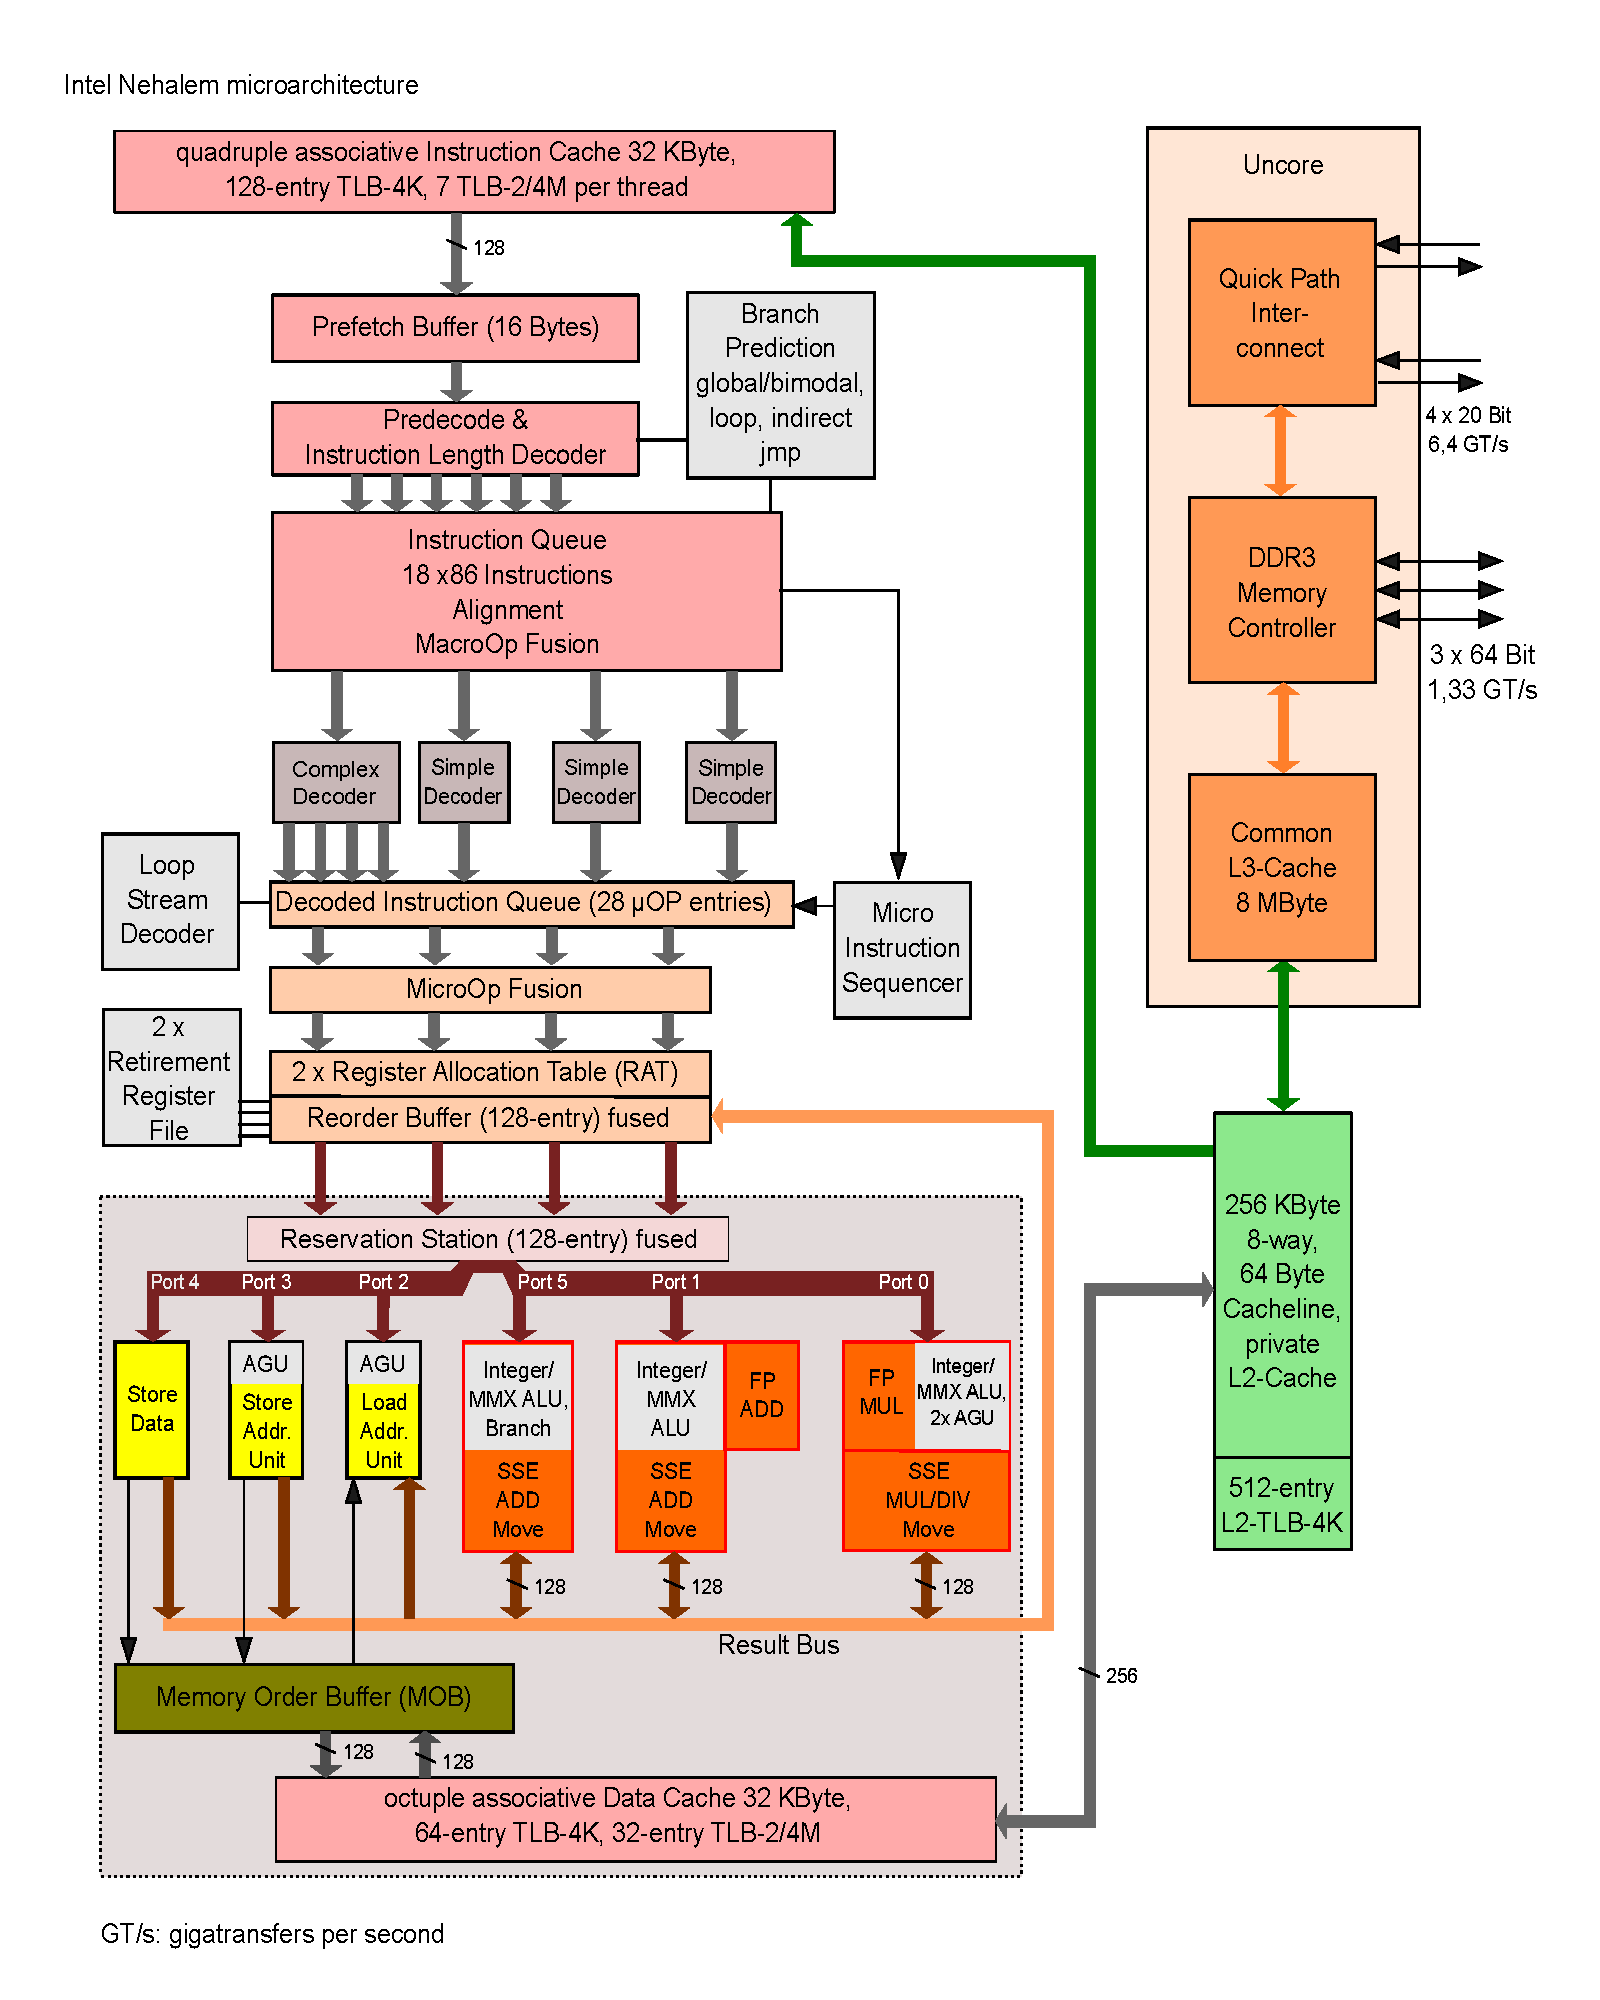
\includegraphics[clip, scale=.26, trim=0 0 0 1.7cm]{Intel_Nehalem_arch}
\end{center}
\end{frame}


\begin{frame}{The Nehalem architecture}
\begin{tikzpicture}[remember picture,overlay]
    \node[xshift=-0.4cm,yshift=-0.3cm] at (current page.center) {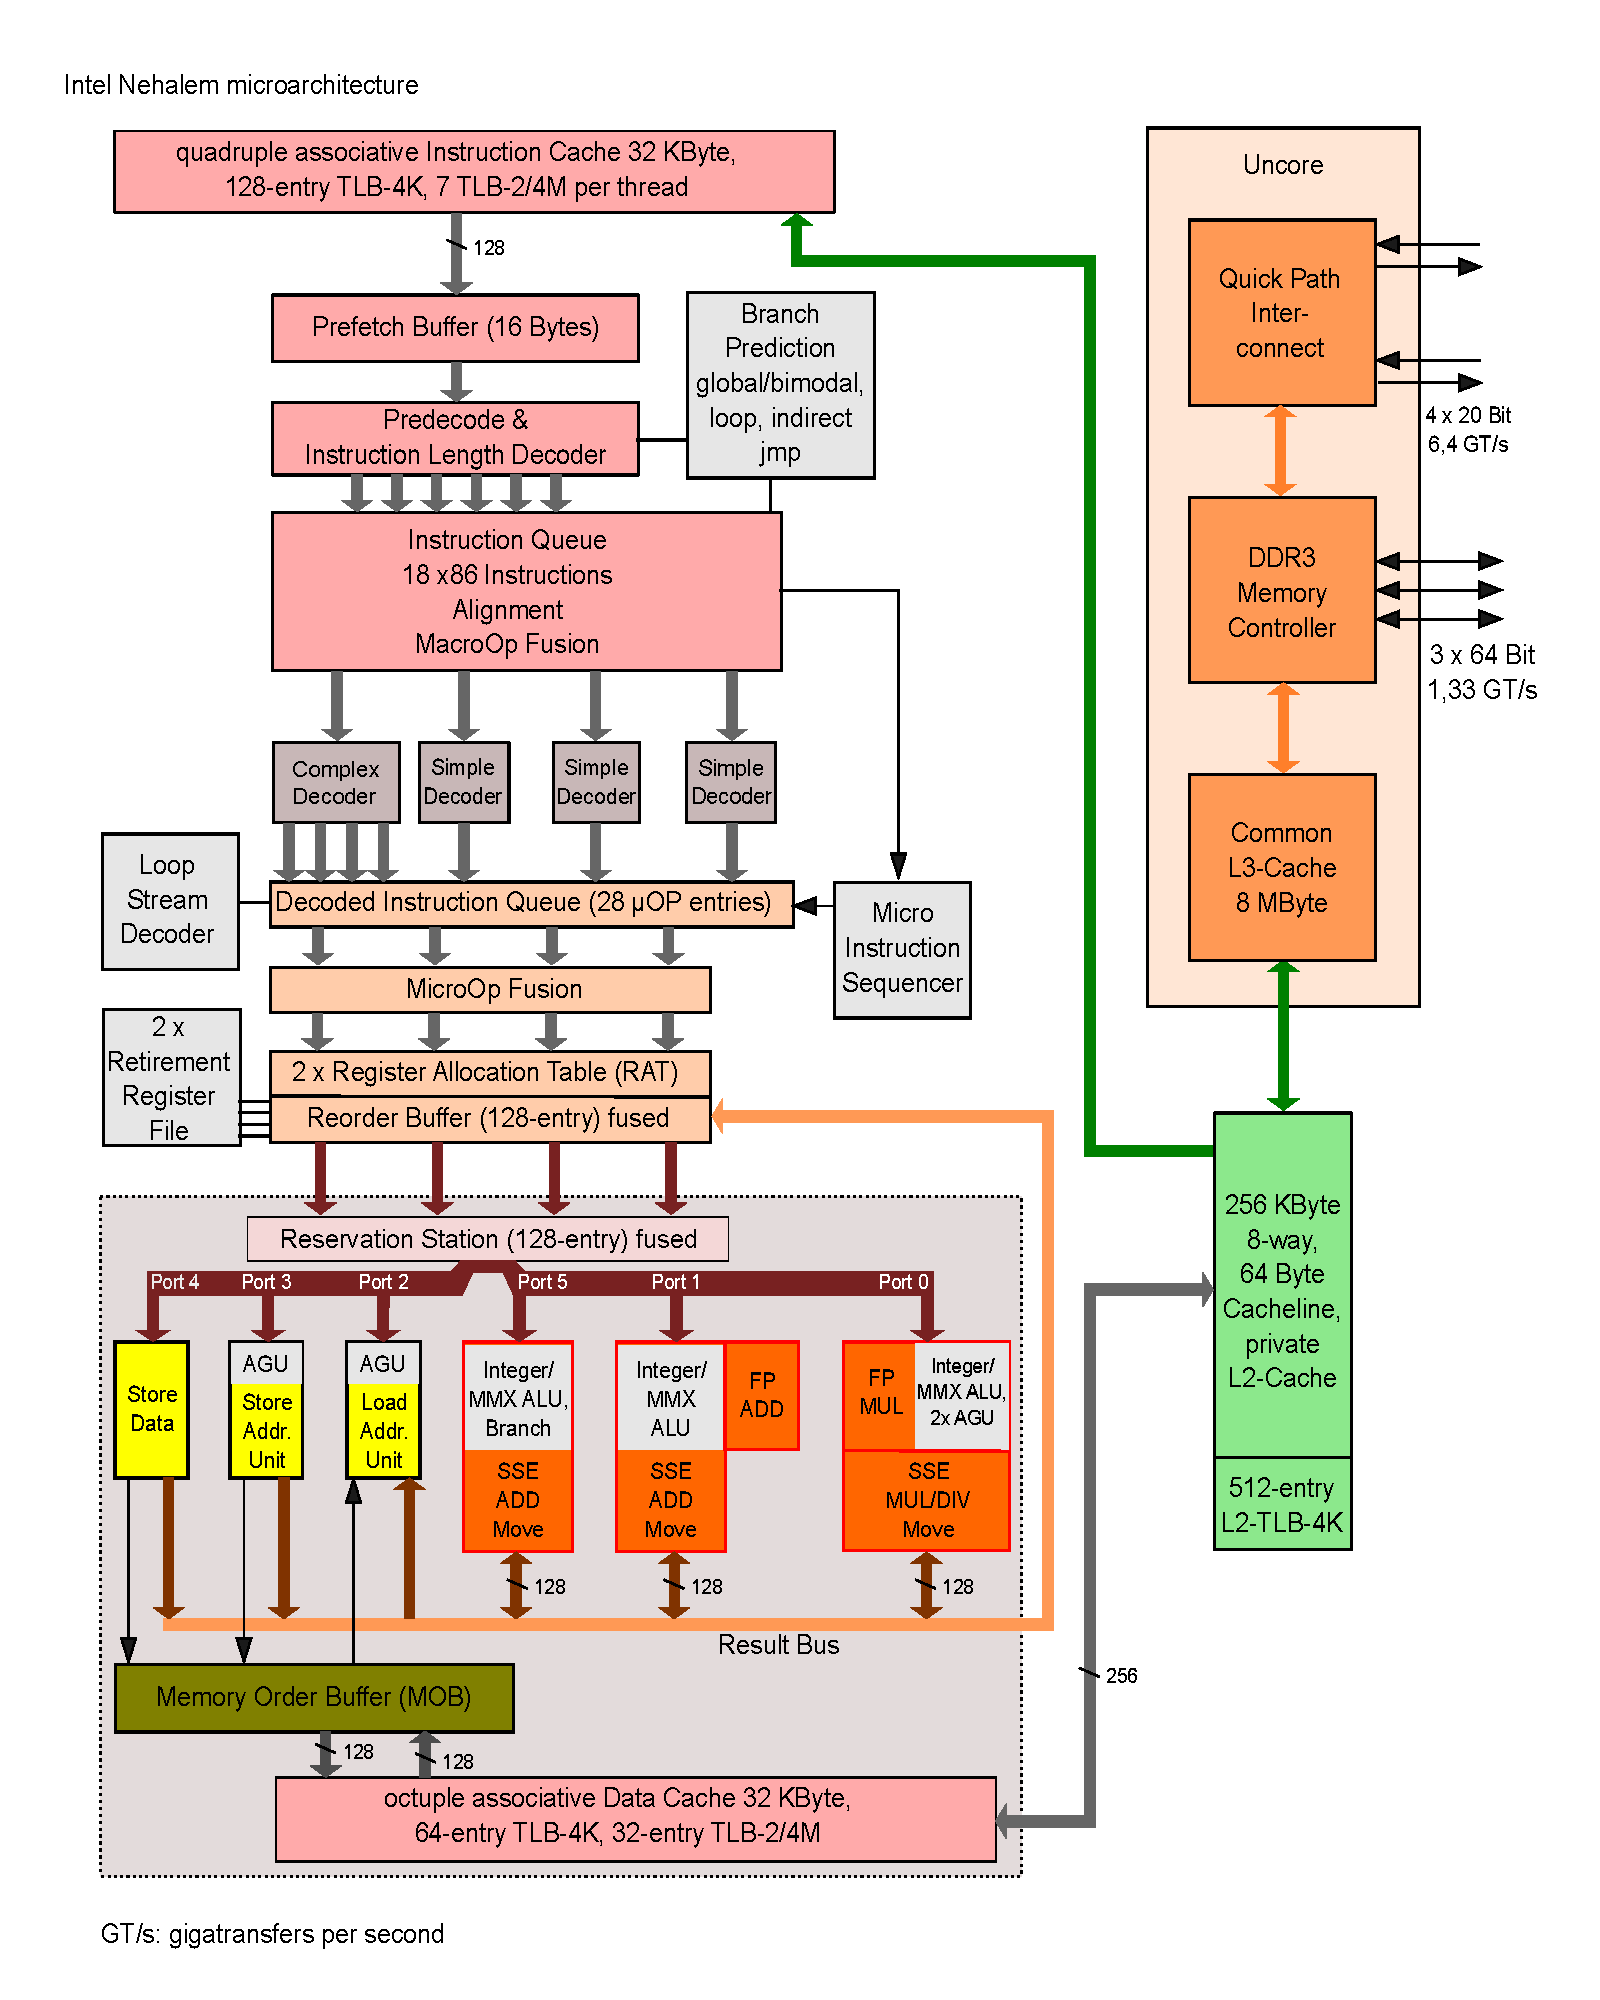
\includegraphics[clip, trim=0.5cm 2cm 9.78cm 20cm, scale=.65]{Intel_Nehalem_arch}};
\end{tikzpicture}
        
\end{frame}

\section{Introduction to IACA}

\begin{frame}{What is IACA?}

\begin{itemize}[<+- | alert@+>]
    \item Intel® Architecture Code Analyzer
    \item Static analysing tool for assembly code (usually a loop) on Intel processors
    \item Computes port pressure and critical path
    \item Allows you to analyze code perfomance on a specific machine!
    \item Provides an estimate of performance\only<6>{, \alert{i.e. no absolute results}}
\end{itemize}

\end{frame}


\begin{frame}[fragile]{How to use IACA?}

\begin{lstlisting}
#include "iacaMarks.h"

int main(void) {
    int a = 3;
    int b = 4;
    
    (*@\textcolor{Green}{IACA\_START}  @*)
    a++;
    b = a * 4;
    (*@\textcolor{Green}{IACA\_END}  @*)
    
    return b;
}
\end{lstlisting}
\end{frame}

\begin{frame}[fragile]{IACAs Output - Reduced}
\begin{itemize}
    \item DV - Divider Pipe
    \item D\phantom{V} - Data fetch pipe
\end{itemize}
\begin{center}
\begin{tabular}{|c|c c|c|c c|c c|c|c|c|c|}
  \hline
  \textbf{Port} & 0 & DV & 1 & 2 & D & 3 & D & 4 & 5 & 6 & 7 \\ \hline
  \textbf{Cycles} & $0.5$ & $0.0$ & $0.5$ & $1.4$ & $1.0$ & $1.4$ & $1.0$ & $2.0$ & $0.5$ & $0.5$ & $1.3$ \\
  \hline
\end{tabular}
\end{center}
\end{frame}

\begin{frame}[fragile]{IACAs Output - Detailled}
\hspace*{-0.6cm}
\resizebox{1.1\textwidth}{!}{
\begin{tabular}{|r|c|c c|c|c c|c c|c|c|c|c|c|}
  \hline
  \multicolumn{1}{|c|}{\multirow{2}{*}{\textbf{Instruction}}}&\textbf{Num Of} & \multicolumn{11}{|c|}{Ports pressure in cycles} &\multirow{2}{*}{\textbf{CP}}\\
  \cline{3-13}
  &$\boldsymbol{\mu}$\textbf{ops} & 0 & DV & 1 & 2 & D & 3 & D & 4 & 5 & 6 & 7 & \\ \cline{1-14}
  add dword ptr [rbp-0x4], 0x1& 4 &  &  & $0.5$ & $1.0$ & $1.0$ & $0.3$ & & $1.0$ & $0.5$ & & $0.6$ & $\surd$ \\
%  \cline{1-13}
  mov eax, dword ptr [rbp-0x4] & 1 &  &  &  &  &  & $1.0$ & $1.0$ &  &  & & & \\
 % \cline{1-13}
  shl eax, 0x2&1 & $0.5$ &  &  &  &  &  &  &  &  & $0.5$ & &  \\
  %\cline{1-13}
  mov dword ptr [rbp-0x8], eax & 2 &  &  &  & $0.3$ &  &  &  & $1.0$ &  & &$0.6$ & $\surd$ \\
  \hline
\end{tabular}
}
\end{frame}



\section{Disadvantages of IACA}

\begin{frame}[fragile]{Disadvantages of IACA}
\begin{itemize}[<+- | alert@+>]
    \item It's closed source
    \item It's not up to date
    \begin{itemize}[<+- | alert@+>]
        \item IACA $2.3$ supports $1^{\text{st}}$ to $6^{\text{th}}$ generation of of Intel Core processors
        \item IACA $3.0$ only supports $4^{\text{th}}$ to $6^{\text{th}}$ generation
        \item The $8^{\text{th}}$ generation was released in 2017
    \end{itemize}
    \item It completely ignores branches
\end{itemize}
\end{frame}

\begin{frame}[fragile]{A branching example}
\begin{verbatim}
1:   mov rax, 1
2:   cmp rcx, 0
3:   jne else
4:   add rbx, rax
5:   jmp end
else:
6:   add rbx, rax
end:
7:   add rbx, rbx
\end{verbatim}
\end{frame}

\begin{frame}[fragile]{The dependency graph}

\begin{minipage}{.35\textwidth}
  \begin{verbatim}
1:   mov rax, 1
2:   cmp rcx, 0
3:   jne else
4:   add rbx, rax
5:   jmp end
else:
6:   add rbx, rax
end:
7:   add rbx, rbx
\end{verbatim}
\end{minipage}% This must go next to `\end{minipage}`
\begin{minipage}{.5\textwidth}
  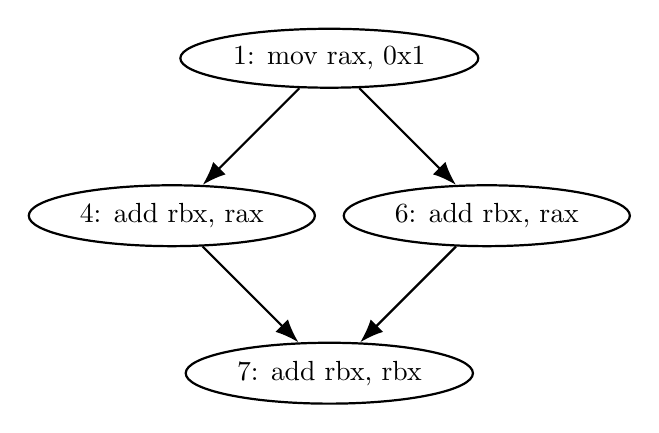
\begin{tikzpicture}
    \node		[draw]		(A)  {1: mov rax, 0x1};
	\node		[]		(W1) [below of=A, below of=A]		{};	
	\node		[draw]		(B)[left of=W1, left of=W1] {4: add rbx, rax};
	\node       [draw]  (C)  [right of=W1, right of=W1] {6: add rbx, rax};
	\node       [draw]  (D)  [below of=W1, below of=W1] {7: add rbx, rbx};
	\draw[-{Latex[length=3mm]}, thick] (A)--(B);
	\draw[-{Latex[length=3mm]}, thick] (A)--(C);
	\draw[-{Latex[length=3mm]}, thick] (B)--(D);
	\draw[-{Latex[length=3mm]}, thick] (C)--(D);
	
\end{tikzpicture}
\end{minipage}


\end{frame}

\begin{frame}[fragile]{IACAs version of the graph}

\begin{minipage}{.35\textwidth}
  \begin{verbatim}
1:   mov rax, 1
2:   cmp rcx, 0
3:   jne else
4:   add rbx, rax
5:   jmp end
else:
6:   add rbx, rax
end:
7:   add rbx, rbx
\end{verbatim}
\end{minipage}% This must go next to `\end{minipage}`
\begin{minipage}{.5\textwidth}
  
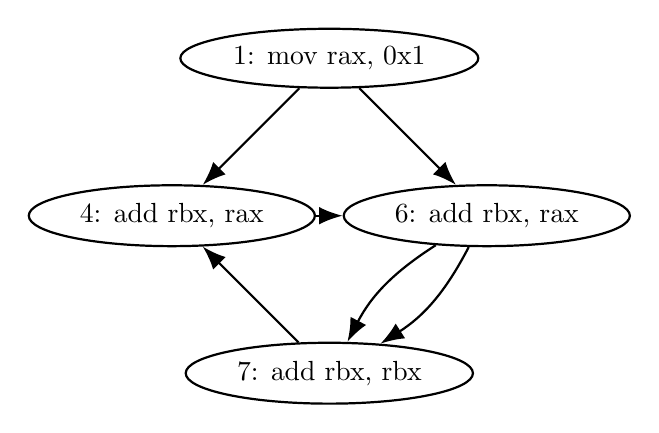
\begin{tikzpicture}
    \node		[draw]		(A)  {1: mov rax, 0x1};
	\node		[]		(W1) [below of=A, below of=A]		{};	
	\node		[draw]		(B)[left of=W1, left of=W1] {4: add rbx, rax};
	\node       [draw]  (C)  [right of=W1, right of=W1] {6: add rbx, rax};
	\node       [draw]  (D)  [below of=W1, below of=W1] {7: add rbx, rbx};
	\draw[-{Latex[length=3mm]}, thick] (A)--(B);
	\draw[-{Latex[length=3mm]}, thick] (A)--(C);
	\draw[-{Latex[length=3mm]}, thick] (D)--(B);
	\draw[-{Latex[length=3mm]}, thick] (B)--(C);
	\draw[-{Latex[length=3mm]}, thick] (C) to [bend right=15](D);
	\draw[-{Latex[length=3mm]}, thick] (C) to [bend left=15](D);
\end{tikzpicture}
\end{minipage}

\end{frame}

\section{My take on it}

\begin{frame}{My take on it}
\textbf{What exactly will I do?}
\begin{itemize}[<+- | alert@+>]
    \item Reimplement the core functionality of IACA
    \item Branch dependencies will be taken into account
    \item My implementation will take measurements of microarchitectures as an input
    \item I.e. you can analyze new Intel Core processors basically on release
\end{itemize}
\end{frame}

\begin{frame}[fragile]{The XML measurement file}
\begin{lstlisting}[language=XML, basicstyle=\ttfamily\scriptsize, breaklines=true]
<instruction ... iform="ADD_LOCK_MEMv_GPRv" ...>
    <operand idx="2" type="reg" ...>RAX,RCX,RDX,RBX,...</operand>
    <operand idx="3" type="flag" ...>OF</operand>
    ...
    <architecture name="NHM">
        <measurement ... port15="2" port2="1" port3="1" port4="1" total_uops="5">
            <latency ... cycles="19" startOp="2" targetOp="3"/>
            ...
        <\measurement>
    </architecture>
<\instruction>
\end{lstlisting}
\end{frame}

\section{Problems I'll be facing}

\begin{frame}{Inaccuracies}
\textbf{I can't know\dots}
\begin{itemize}[<+- | alert@+>]
    \item which algorithm the ``reservation station'' uses
    \item about the dependencies between $\mu$ops
\end{itemize}
\only<3->{\textbf{Also\dots}}
\begin{itemize}[<+- | alert@+>]
    \item it is very hard to compute latency under non-optimal conditions
    \item some instruction's "iforms" are incomplete in the XML file
\end{itemize}
\end{frame}


{\setbeamercolor{palette primary}{fg=white, bg=black}
\begin{frame}[standout]
  Thank you for your attention!\\
  Questions?
\end{frame}
}


\begin{frame}{References}

  \bibliography{zitate}
  \bibliographystyle{siam}

\end{frame}






\end{document}
